\documentclass[12pt]{article}
\usepackage{graphicx}
\graphicspath{ {images/} }
\usepackage[margin=1in]{geometry}
\usepackage{float}
\title{Propagation of Voltage in a Neuron: The Cable Equation}
\author{Darice Guittet, Elise Niedringhaus, Sarah Liddle}

\begin{document}
\maketitle
\section{Introduction}

Information within the brain is transmitted between neurons largely due to action potentionals, otherwise known as spikes, which are when the voltage in a neuron rapidly rises and falls. These allow communication between brain cells. A.L Hodgkin and A.F. Huxley received a 1963 Nobel Prize for their work regarding this topic, specifically the discovery that individual parts of the axonal membrane behave similarly to a component in an electric circuit. With this knew knowledge, it is now possible to derive equations that represent the voltage propagation in a neuron using formulas similar to those that describe current, resistance, and voltage in an electrical system. This pattern of diffusion along the membrane of neurons by current or voltage is called cable theory, which is what we will be analyzing in this report.

\subsection{Understanding the Model}
The model we are using to understand the propogation of voltage in a neuron can be described by the following partial differential equation:
\begin{equation} \label{1}
\frac{\partial{v(x,t)}}{\partial{t}}=\frac{\partial^2{v(x,t)}}{\partial{x}^2}+f(v(x,t))
\end {equation}
The terms with partial derivatives are from the heat or diffusion equation, mathematically describing the process when molecules move from areas of high concentration to places of low concentration. The $f(v(x,t))$ term accounts for ion channels in a neuron; these open and close to add or decrease from the ions entering the cell based on its current voltage. 


Therefore, the final partial differential equation we will be using to analyze voltage propagation in a neuron is:
\begin{equation} \label{2}
\frac{\partial{v(x,t)}}{\partial{t}}=\frac{\partial^2{v(x,t)}}{\partial{x}^2}+f(v(x,t))+J_{ext}(x,t)
\end {equation}

\subsection{Purpose}
In this project, we aim to examine the partial differential equation model of this phenomenon to analyze the propagation of action potentials throughout a neoron. First, we will look at a passive membrane where there is no voltage gradient and ions will leak out of the cell by first solving the stationary solution and then solving the partial differential equation inorder to analyze the impulse propagation reaction to various initial voltage inputs. Next, we will analyze a nonlinear model that takes into account that membrane ion channels often have a "two state" nature--meaning... We will examine the traveling wave solutions of this model. Therefore, we aim to have a better understanding of how voltage propagates within under various conditions and inputs.


\section{Numerical Solutions}
After analytically solving the voltage equation, we also found numerical solutions. In order to numerically solve for this partial differential equation, we must first discretize both partial derivatives. For this problem, discretization is the process of using Taylor series to approximate the first time derivative of the voltage function in terms of the point we will approximate and the known point one time step before it, like so:
\[\frac{\partial{v(x,t)}}{\partial{t}}=\frac{v^{j+1}_i-v^j_i}{\Delta{t}}+O(\Delta{t})\]
In this equation, $v^j_i$ represents the point at $x=x_i$ and $t=t_j$ and $O(\Delta{t})$ represents the order of the error of this approximation, meaning that the error is a function of the size of the timestep.
Using the same approach, we will use Taylor series to write the second x derivative of the voltage function in terms of three known points, like so:
\[\frac{\partial^2{v(x,t)}}{\partial{x}^2}=\frac{v^{j}_{i+1}-2v^j_i+v^j_{i-1}}{(\Delta{x})^2}+O((\Delta{x})^2)\]
Using these two formulas and putting these into our original PDE gives:
\[\frac{v^{j+1}_i-v^j_i}{\Delta{t}}=\frac{v^{j}_{i+1}-2v^j_i+v^j_{i-1}}{(\Delta{x})^2}-v^j_i+J_{ext}(x,t)\]
Finally, we can algebraically solve this equation for $v^{j+1}_i$, in terms of values that are known. Therefore, going timestep by timestep starting from the initial condition, this question can be usedto solve numerically for the entire subset of the neuron we're examining. Note that I have removed the $J_{ext}(x,t)$ form from this equation
\begin{equation} \label{*}
v^{j+1}_i=\frac{\Delta{t}}{(\Delta{x})^2}(v^{j}_{i+1}+v^{j}_{i-1})+(1-\frac{\Delta{t}(2+(\Delta{x})^2)}{(\Delta{x})^2})v^{j}_{i}+\Delta{t}*J_{ext}(x,t)
\end {equation}
However, looking at the $v^{j}_{i}$ term in this equation, it can be seen that if $\frac{\Delta{t}(2+(\Delta{x})^2)}{(\Delta{x})^2}>1$ then this approximation is unstable and will not converge. Therefore, in order for this method of finite difference approximation to converge, $\Delta{t}$ must be much smaller than $(\Delta{x})^2$ 
When using equation (\ref{*}) to approximate this solution numerically, we will be using $J_{ext}(x,t)=10e^{-25x^2}\delta{(t)}$. However, instead of simulating the function $\delta{(t})$, we will remove $J_{ext}(x,t)$ from the function representing the numerical function and use it as the initial condtion, making $v(x,0)=10e^{-25x^2}$. The boundary conditions will be zero everywhere else. Since we cannot approximate an infinite interval of x and t, we will instead look at the region from $[-10,10]$ for x and $[0,50]$ for t. 
First, using the given $\Delta{t}=0.1$ and $\Delta{x}=0.1$, we can see the the approximation does not converge to a solution, as predicted, and that it is unstable. 
\begin{figure}[H]
  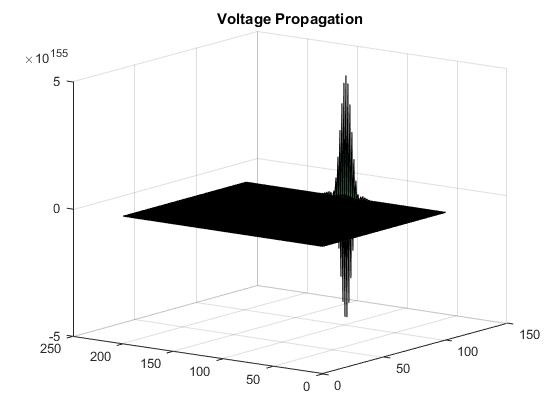
\includegraphics[width=\linewidth]{plot1.jpg}
  \caption{Plot of Unstable Numerical Approximation}
  \label{fig:sketch1}
\end{figure}
In this figure, we had to shorten the total time to 10 seconds because by time fifty, the instability casued parts of the solutions to approach infinity, so Matlab was not able to plot it reasonably. One can see in this plot that as time increases, the voltage increases exponentially higher than it began. \par
Next, when we change $\Delta{t}$ to 0.001 the meet the conditions for stability of this approximation, we can see that the approximation closely resembles our analytic solution to this partial differential equation.
\begin{figure}[H]
  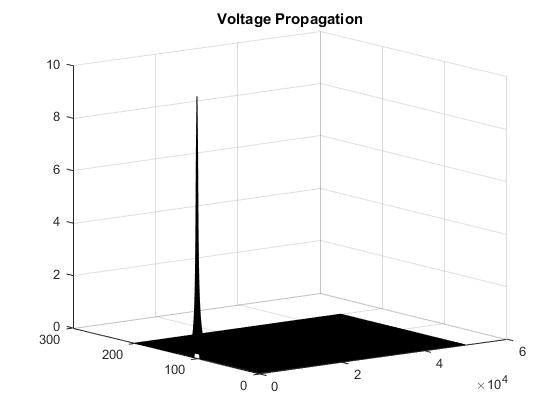
\includegraphics[width=\linewidth]{Plot2.jpg}
  \caption{Plot of Stable Numerical Approximation}
  \label{fig:sketch2}
\end{figure}
As one can see, this plot is matches closely to the analytical solution. It shows the spike of voltage at $t=0$ and $x=0$ and demonstrates how that voltage propagates throughout the neuron, approaching zero as time and x increases. 







\end{document}